\chapter{Конструкторская часть}

\section{Концептуальный дизайн}

Для описания функциональной модели системы используется нотация IDEF0. На рисунке \ref{fig:idef0-0} приведена верхнеуровневая модель системы бронирования автомобилей. На рисунке \ref{fig:idef0-1} представлена декомпозиция основных процессов: регистрация и авторизация, просмотр автомобилей, бронирование, оплата и сбор статистики.

\begin{figure}[h!]
	\begin{center}
		\resizebox{\textwidth}{!}{
		\begin{tikzpicture}[
			process/.style={draw, rectangle, minimum width=7.5cm, minimum height=3.2cm, align=center, line width=0.8pt},
			arrow/.style={-{Latex[length=3mm]}, line width=0.8pt},
			label/.style={align=center, font=\small}
		]
			\node[process] (system) {Система бронирования\\автомобилей};
			\node[label, left=2.7cm of system] (input) {Запросы пользователей:\\регистрация, вход,\\поиск и бронирование};
			\node[label, right=2.7cm of system] (output) {Бронирования, платежи,\\список автомобилей,\\административная статистика};
			\node[label, above=1.7cm of system] (control) {Требования ТЗ, OIDC/JWT,\\правила ролей Admin/User,\\ограничения Kubernetes};
			\node[label, below=1.7cm of system] (mechanism) {React UI, FastAPI-сервисы,\\PostgreSQL, Kafka, Helm, Ingress};
			\draw[arrow] (input) -- (system);
			\draw[arrow] (system) -- (output);
			\draw[arrow] (control) -- (system);
			\draw[arrow] (mechanism) -- (system);
		\end{tikzpicture}}
		\caption{Концептуальная модель системы в нотации IDEF0}
		\label{fig:idef0-0}
	\end{center}
\end{figure}

\begin{figure}[h!]
	\begin{center}
		\resizebox{\textwidth}{!}{
		\begin{tikzpicture}[
			process/.style={draw, rectangle, minimum width=3.4cm, minimum height=1.5cm, align=center, line width=0.8pt},
			arrow/.style={-{Latex[length=2.5mm]}, line width=0.8pt},
			note/.style={align=center, font=\small}
		]
			\node[process] (auth) {A1\\Регистрация\\и авторизация};
			\node[process, right=1.1cm of auth] (cars) {A2\\Просмотр\\автомобилей};
			\node[process, right=1.1cm of cars] (rent) {A3\\Бронирование\\на даты};
			\node[process, right=1.1cm of rent] (pay) {A4\\Создание\\платежа};
			\node[process, below=1.3cm of rent] (stats) {A5\\Сбор\\статистики};
			\node[note, left=1.7cm of auth] (user) {Пользователь\\или администратор};
			\node[note, right=1.7cm of pay] (result) {Подтвержденное\\бронирование\\и отчет};
			\node[note, above=1.0cm of rent] (rules) {JWT, роли, JWKs,\\правила доступности авто};
			\node[note, below=1.0cm of stats] (infra) {Kafka, PostgreSQL,\\Kubernetes};
			\draw[arrow] (user) -- (auth);
			\draw[arrow] (auth) -- node[above, font=\scriptsize]{JWT} (cars);
			\draw[arrow] (cars) -- node[above, font=\scriptsize]{выбранный автомобиль} (rent);
			\draw[arrow] (rent) -- node[above, font=\scriptsize]{сумма} (pay);
			\draw[arrow] (pay) -- (result);
			\draw[arrow] (rent) -- (stats);
			\draw[arrow] (pay) |- (stats);
			\draw[arrow] (rules) -- (auth);
			\draw[arrow] (rules) -- (rent);
			\draw[arrow] (infra) -- (stats);
		\end{tikzpicture}}
		\caption{Детализированная концептуальная модель системы в нотации IDEF0}
		\label{fig:idef0-1}
	\end{center}
\end{figure}

\clearpage
\section{Сценарии функционирования системы}

\textbf{Регистрация пользователя}
\begin{enumerate}
	\item Пользователь открывает веб-интерфейс и выбирает режим регистрации.
	\item Пользователь вводит логин, email, имя и пароль.
	\item UI отправляет запрос на регистрацию в gateway-service.
	\item Gateway-service передает запрос в identity-service.
	\item Identity-service проверяет уникальность логина и email, сохраняет пользователя с ролью User и возвращает результат.
	\item Пользователь получает сообщение об успешном создании аккаунта и может выполнить вход через Identity Provider.
\end{enumerate}

\textbf{Авторизация пользователя}
\begin{enumerate}
	\item Пользователь нажимает кнопку входа в веб-интерфейсе.
	\item UI формирует запрос Authorization Code Flow и перенаправляет пользователя на \texttt{/oauth/authorize}.
	\item Identity Provider показывает форму входа.
	\item После ввода логина и пароля Identity Provider создает authorization code и перенаправляет пользователя на callback UI.
	\item UI через gateway-service обменивает authorization code на JWT.
	\item JWT сохраняется в браузере и используется в последующих API-запросах.
\end{enumerate}

\textbf{Бронирование автомобиля}
\begin{enumerate}
	\item Пользователь выбирает даты начала и окончания аренды.
	\item Пользователь выбирает доступный автомобиль и нажимает кнопку бронирования и оплаты.
	\item UI отправляет запрос в gateway-service с идентификатором автомобиля и выбранными датами.
	\item Gateway-service валидирует JWT и получает информацию об автомобиле из cars-service.
	\item Gateway-service резервирует автомобиль, изменяя его доступность.
	\item Gateway-service создает платеж в payment-service.
	\item Gateway-service создает запись бронирования в rental-service.
	\item Gateway-service отправляет событие о бронировании в Kafka.
	\item UI отображает пользователю созданное бронирование и статус платежа.
\end{enumerate}

\textbf{Завершение бронирования}
\begin{enumerate}
	\item Пользователь открывает страницу своих бронирований.
	\item Пользователь нажимает кнопку завершения активной аренды.
	\item Gateway-service получает данные бронирования из rental-service.
	\item Gateway-service освобождает автомобиль через cars-service.
	\item Gateway-service меняет статус бронирования на FINISHED через rental-service.
	\item Gateway-service отправляет событие в Kafka.
\end{enumerate}

\textbf{Отмена бронирования}
\begin{enumerate}
	\item Пользователь открывает список бронирований.
	\item Пользователь нажимает кнопку отмены.
	\item Gateway-service освобождает автомобиль.
	\item Gateway-service меняет статус бронирования на CANCELED.
	\item Gateway-service отменяет платеж или помещает операцию отмены в очередь повторной обработки при недоступности платежного сервиса.
	\item Gateway-service отправляет событие об отмене в Kafka.
\end{enumerate}

\textbf{Просмотр статистики администратором}
\begin{enumerate}
	\item Администратор проходит авторизацию.
	\item UI отображает вкладку администрирования.
	\item Администратор открывает отчет статистики.
	\item Gateway-service проверяет наличие роли Admin в JWT.
	\item Gateway-service запрашивает данные у statistics-service.
	\item UI отображает сводку и последние события.
\end{enumerate}

\section{Диаграммы прецедентов}

В системе выделены 3 роли: неавторизованный пользователь, авторизованный пользователь и администратор. На рисунках \ref{fig:use-case-non-auth}-\ref{fig:use-case-admin} представлены диаграммы прецедентов для каждой роли.

\begin{figure}[H]
	\begin{center}
		{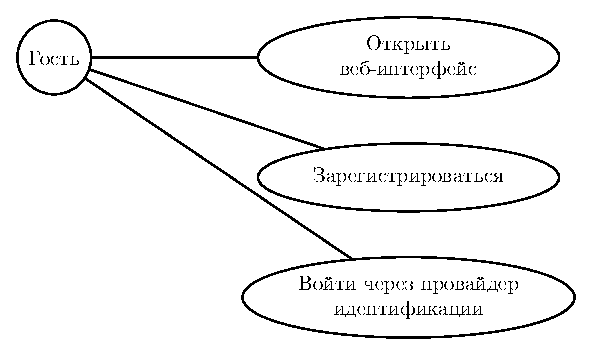
\includegraphics[width=0.82\textwidth]{../img/use-case/non-auth-user.pdf}}
		\caption{Диаграмма прецедентов с точки зрения неавторизованного пользователя}
		\label{fig:use-case-non-auth}
	\end{center}
\end{figure}

\begin{figure}[H]
	\begin{center}
		{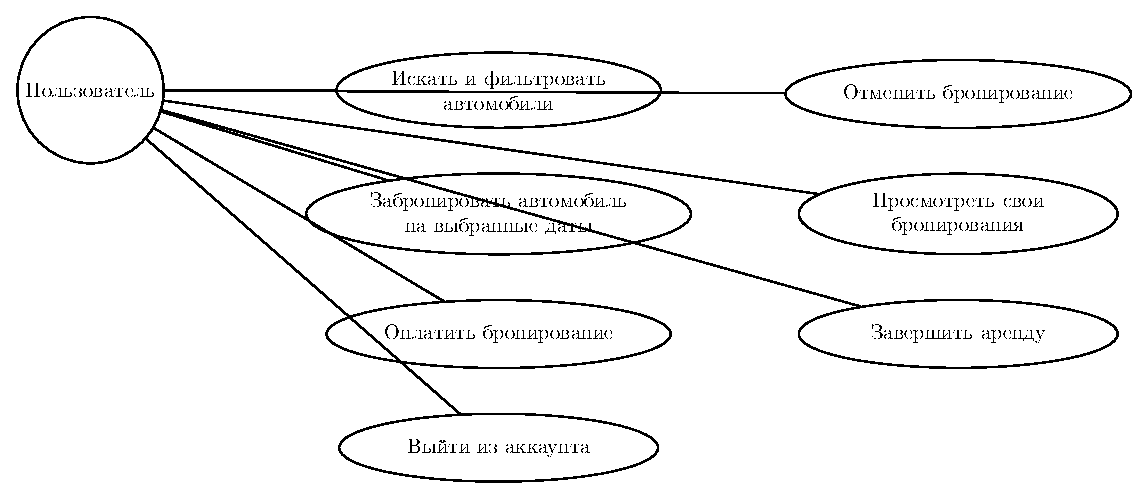
\includegraphics[width=\textwidth]{../img/use-case/auth-user.pdf}}
		\caption{Диаграмма прецедентов с точки зрения авторизованного пользователя}
		\label{fig:use-case-auth}
	\end{center}
\end{figure}

\begin{figure}[H]
	\begin{center}
		{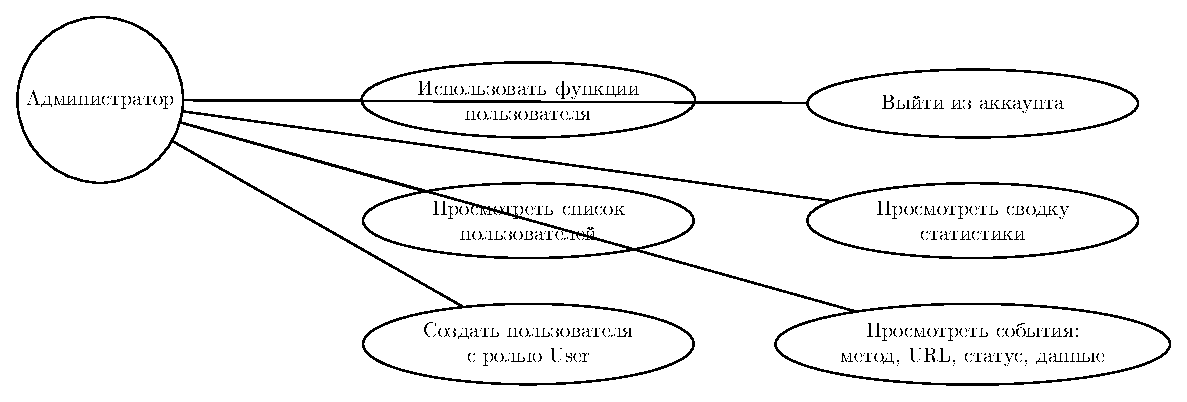
\includegraphics[width=\textwidth]{../img/use-case/admin.pdf}}
		\caption{Диаграмма прецедентов с точки зрения администратора}
		\label{fig:use-case-admin}
	\end{center}
\end{figure}

\section{Архитектура микросервисов}

В системе используется микросервисная архитектура. Клиентское приложение обращается к gateway-service, который агрегирует запросы и скрывает внутреннюю структуру системы. Внутренние сервисы не публикуются наружу напрямую.

Основной поток данных при бронировании включает cars-service, payment-service и rental-service. События пользовательских действий отправляются в Kafka, после чего statistics-service обрабатывает их и сохраняет для последующего отображения администратору.

\section{Проектирование авторизации}

Identity-service реализует следующие функции OpenID Connect:

\begin{itemize}
  \item endpoint авторизации \texttt{/oauth/authorize};
  \item endpoint обмена кода на токен \texttt{/oauth/token};
  \item metadata \texttt{/.well-known/openid-configuration};
  \item endpoint JWKs \texttt{/oauth/jwks};
  \item scopes \texttt{openid}, \texttt{profile}, \texttt{email}.
\end{itemize}

JWT содержит сведения о пользователе, email, имени и ролях. Сервисы получают JWKs от Identity Provider и валидируют токены без дополнительного запроса к нему при каждом пользовательском действии.

\section{Вывод}

В конструкторской части были описаны основные сценарии работы системы, роли пользователей, архитектура микросервисов и механизм авторизации на основе OpenID Connect и JWT.
